% !TEX root = ../../Tesi.tex

%******************************************
%	Resoconto dello stage
%******************************************

\chapter{Resoconto dello stage}
\label{cap:resoconto_dello_stage}

	\section{Individuazione dei motori di ricerca}
	Ad oggi, sono disponibili in rete un gran numero di motori di ricerca, sia proprietari, sia \gls{open source}. Questi, mettono a disposizione funzionalità di ricerca più o meno avanzate e, a seconda di vari fattori come possono essere, ad esempio, la tipologia e la quantità di dati che vogliamo indicizzare, rendendoli ricercabili agli utenti, possiamo optare per l'uno piuttosto che per l'altro. \\
	La scelta del motore di ricerca più adatto alle specifiche esigenze, non è questione affatto banale; molte volte esistono varie soluzioni in grado di modellare bene il problema che dobbiamo affrontare, simili tra loro, che differiscono però per alcuni aspetti chiave. \\
	Focalizzando l'attenzione sulle esigenze dettate dai siti informativi Camerali, possiamo già applicare un primo filtro sui motori di ricerca da utilizzare: motori di ricerca proprietari \textit{vs} motori di ricerca \gls{open source}. \\
	Un motore di ricerca proprietario rappresenta indubbiamente un onere per l'azienda e, oltre a ciò, quest'ultima non ha il pieno controllo sulla destinazione finale dei dati; queste questioni non si hanno invece in un sistema \gls{open source}, nel quale il codice sorgente è liberamente modificabile e analizzabile, avendo dunque il pieno controllo sull'intero sistema. \\
	Nella figura 3.1 è presente una classifica dei motori di ricerca, aggiornata a Novembre 2017, calcolata su parametri che rappresentano la popolarità del sito (maggiori informazioni sui punteggi assegnati sono disponili al seguente indirizzo: \url{https://db-engines.com/en/ranking_definition}). Da questa tabella, notiamo come in testa alla classifica siano presenti tre motori di ricerca che hanno un ampio margine di distacco, in termini di punteggio ad essi attribuito, rispetto alle tecnologie che li precedono. Di questi, solamente i primi due (\gls{Solr} e \gls{ElasticSearch}) sono alternative \gls{open source}. \\
	Oltre a ciò, per entrambi i motori di ricerca appena citati, sono disponibili \glspl{Modulo} \gls{Drupal} che rendono possibile la semplice integrazione tra i motori di ricerca e il \gls{CMSg} di interesse. \\
	Le motivazioni appena descritte, hanno così portato alla selezione di \gls{Solr} e \gls{ElasticSearch} come motori di ricerca da studiare nell'ambito dello stage.

	\begin{figure}[htbp]
		\begin{center}
			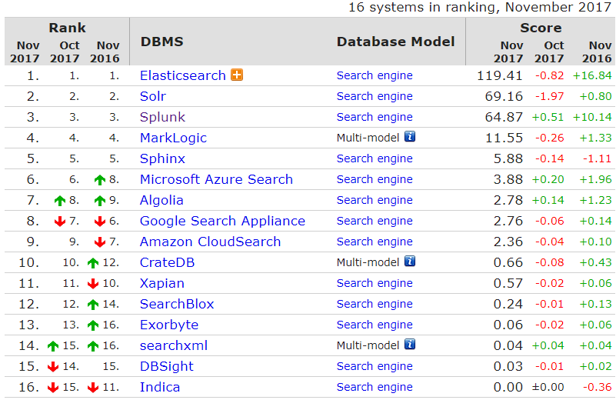
\includegraphics[width=13cm]{tabella_SE}
			\captionof{figure}{\cite{site:confronto_SE}}
		\end{center}
	\end{figure}
	
	\section{Pianificazione}
	Durante la stesura del Piano di Lavoro, assieme al tutor aziendale, ho concordato le attività principali da svolgere durante il periodo di stage, della durata di circa 300 ore, previsto dal mio corso di laurea. Nel documento sopracitato, sono inoltre contenute le \gls{Milestone} pianificate, così come descritto nella \hyperref[subsub:milestone]{sezione 2.2.2, sotto alla voce "Le milestone"}. \\
	Oltre al resoconto quotidiano con il tutor aziendale, al completamento di ogni attività, abbiamo fatto il punto della situazione sullo stato di avanzamento del lavoro, rivedendo e integrando, quando necessario, gli obiettivi settimanali previsti dal Piano di Lavoro. Questa modalità di operare mi ha permesso di rispettare le attività pianificate fin dall'inizio, oltre ad ampliare lo studio delle funzionalità di ricerca offerte da \gls{Drupal}, non inizialmente previste, necessarie però a fornire un quadro più dettagliato sull'intero ambito di lavoro.
	Nell'ultima settimana lavorativa, l'azienda ha inoltre richiesto una presentazione, esposta verbalmente e corredata da diapositive illustrative, sul lavoro operato durante lo stage e sulle relative conclusioni. Più nel dettaglio, nella presentazione ho presentato: scopo e motivazioni del lavoro svolto; come ho organizzato il mio lavoro; funzionalità offerte dalle tecnologie da me esaminate (di interesse per l'azienda); conclusione soggettiva su quale tecnologia sia più adatta nell'ambito dei siti camerali, con suggerimenti per migliorare le funzionalità di ricerca dei suddetti siti; benefici immediati e a lungo termine che il lavoro svolto durante lo stage ha apportato all'azienda; ulteriori ambiti da esplorare, relativamente a queste tecnologie; valutazione soggettiva, mia e del tutor aziendale, riguardo allo stage come esperienza. \\
	
	\section{I siti istituzionali delle Camere di Commercio}

		\subsection{Funzionalità di ricerca attuali}
		Quando un utente visita un sito web, è fondamentale che le informazioni in esso contenute siano facilmente trovabili dall'utente.
		A tal fine, è necessario che un sito web informativo fornisca all'utente strumenti che lo aiutino a trovare agevolmente, in pochi click, quello che sta cercando. La ricerca interna, spesso presente nei siti web, è uno di questi strumenti ed è strettamente legato ai concetti di:
		\begin{itemize}
			\item[--]{\textbf{efficienza}: il numero di azioni da che l'utente deve compiere per trovare quello che sta cercando dev'essere molto limitato; inoltre, i tempi di risposta devono essere molto brevi, quasi impercettibili agli occhi dell'utente, stando dunque nell’ordine dei msec;}
			\item[--]{\textbf{efficacia}: l’utente deve essere in grado di trovare sempre quello che cerca; lo strumento di ricerca deve cercare di avvicinarsi a comprendere quanto più possibile il linguaggio naturale con il quale l'utente comunica al sito web.}
		\end{itemize}
		
		Il fine ultimo dello stage consiste nel cercare di migliorare le funzionalità di ricerca offerte agli utenti, degli attuali siti web istituzionali delle Camere di Commercio. \\
		Prendiamo come esempio l’attuale sito istituzionale della Camera di Commercio di Verona (\cite{site:vr_camerale}): come presentato nella \hyperref[img:conferenze]{figura 3.2}, a fronte della ricerca del termine “Conferenze”, lo strumento di ricerca interno non trova alcun risultato, a differenza invece della ricerca di “Conferenza”, presentato nella \hyperref[img:conferenza]{figura 3.3}, che produce invece alcuni risultati. Rispetto alla prima ricerca effettuata, abbiamo semplicemente cambiato la forma del termine ricercato, dal plurale della prima ricerca al singolare della seconda. \\ 
		Da questo comportamento, possiamo dunque trarre la conclusione che la ricerca viene attuata sui termini esatti, ed è ben lontana dal comprendere i linguaggi naturali.

		\begin{figure}[htbp]
			\label{img:conferenze}
			\begin{center}
				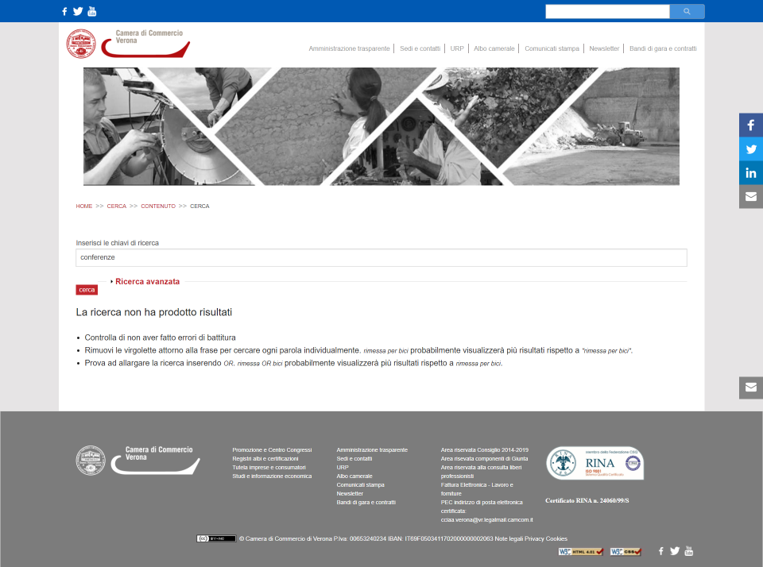
\includegraphics[width=13cm]{vr_attuale}
				\captionof{figure}{\cite{site:vr_attuale}}
			\end{center}
		\end{figure}
	
		\begin{figure}[htbp]
			\label{img:conferenza}
			\begin{center}
				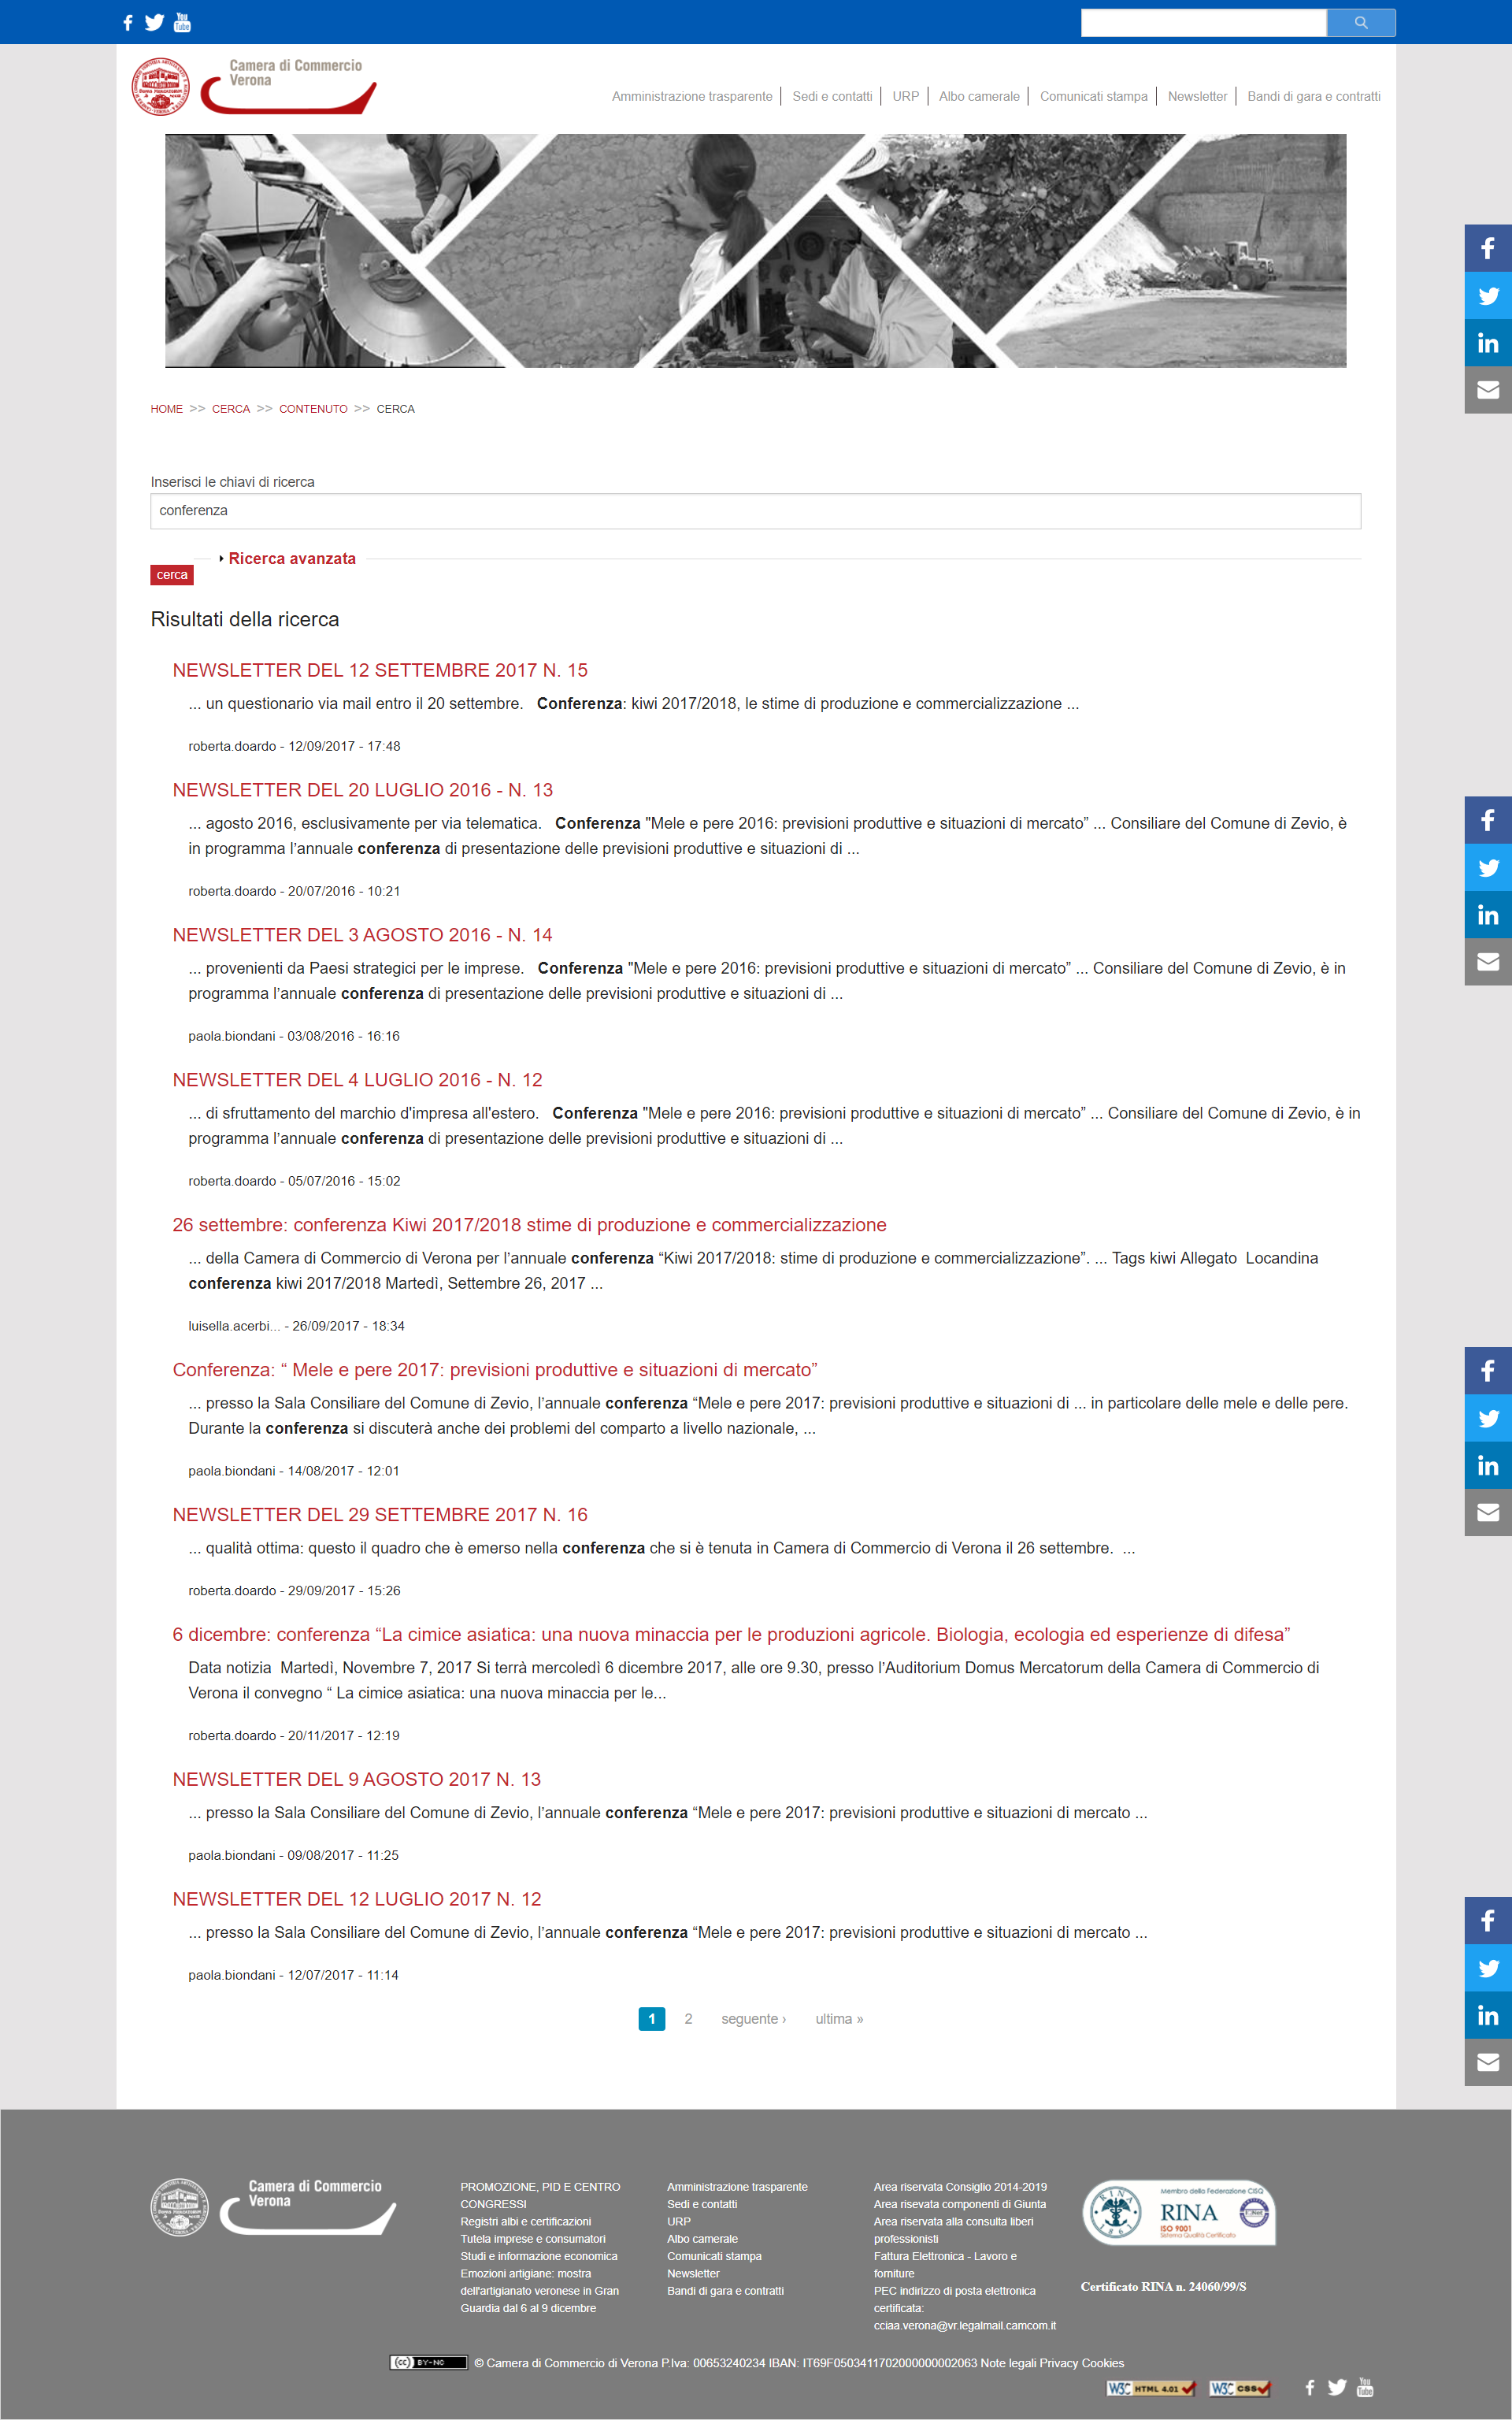
\includegraphics[width=13cm]{vr_attuale_conferenza}
				\captionof{figure}{\cite{site:vr_attuale_conferenza}}
			\end{center}
		\end{figure}
		
		\newpage
		\subsection{Possibile evoluzione}
		\label{sub:possibile_evoluzione}
		Come ho illustrato nella sezione precedente, le funzionalità di ricerca attuali sono molto limitate, ben lontane dal fornire all'utente un'esperienza di navigazione incentrato sulla ricerca, con strumenti limitati nel numero e nella qualità delle funzionalità offerte. \\
		Come possiamo dunque migliorare la ricerca nei siti informativi Camerali?
		Per perseguire questo obiettivo ambizioso, pensiamo alle funzionalità di ricerca con cui gli utenti sono soliti interagire. \\		
		Google ad esempio, mette a disposizione diverse funzionalità che aiutano l’utente ad effettuare una ricerca che produca i risultati attesi, pur gestendo un'enorme quantità di dati. I siti di e-commerce utilizzano inoltre un altro strumento molto utile per una ricerca, che consente agli utenti di filtrare le ricerche, restringendo molto rapidamente i possibili contenuti di interesse: le facets, detti anche filtri multipli, che verranno presentati nel seguito di questo paragrafo. Alcune di queste funzionalità potrebbero essere prese come punto di partenza per migliorare la ricerca interna dei siti informativi Camerali. In particolare:
		
			\subsubsection{Completamento automatico}
			Questa caratteristica consente agli utenti di visualizzare una lista di termini suggeriti sulla base dei caratteri che hanno digitato fino a quel momento; in questo modo, viene ridotto il numero di errori di digitazione della keywords da ricercare, consentendo così ricerche più vicine a quanto pensato dagli utenti, avvicinandosi in tal modo alle loro esigenze. \\ Ulteriore vantaggio è dato dalla riduzione del tempo richiesto agli utenti per effettuare una ricerca, in quanto se questa è presente tra le keywords suggerite, l'utente può risparmiare tempo semplicemente selezionando il suggerimento completo, piuttosto di dover digitare interamente i termini da ricercare, rendendo così la ricerca maggiormente efficiente in termini temporali.
			\begin{figure}[htbp]
				\begin{center}
					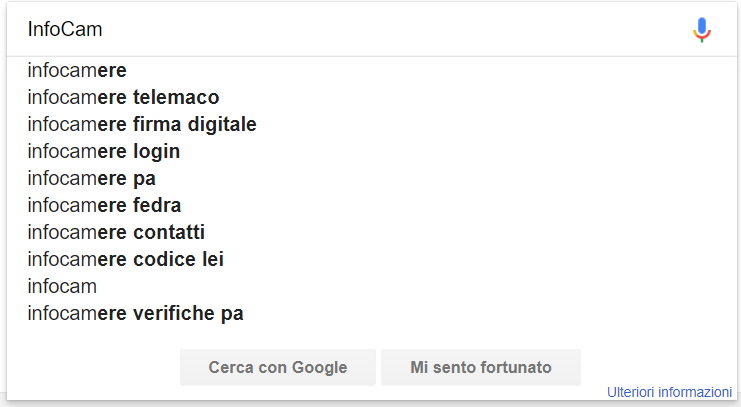
\includegraphics[width=7cm]{completamento_automatico}
					\captionof{figure}{Funzionalità di completamento automatico di Google}
				\end{center}
			\end{figure}
		
			\subsubsection{Paginazione e ordinamento}
			La funzionalità di paginazione permette di rendere le ricerche più rapide, restituendo un sottoinsieme dei risultati di ricerca.
			L'ordinamento consente invece di ordinare i risultati restituiti a seguito di una ricerca, sulla base di specifiche caratteristiche dei documenti indicizzati.
			
			\subsubsection{Controllo ortografico}
			Funzionalità indispensabile per comprendere quanto più possibile il linguaggio naturale con il quale l'utente comunica, il controllo ortografico può essere gestito come:
			\begin{itemize}
				\item {Correzione automatica: viene eseguito automaticamente il controllo ortografico dei termini ricercati, sulla base del fatto che il termine contenente errori ortografici sia indicizzato;}
				\item {"Did you mean...?": vengono suggerite ricerche che potrebbero produrre risultati migliori; l'utente visualizzerà l'elenco di questi suggermenti.}
			\end{itemize}

			\begin{figure}[htbp]
				\begin{center}
					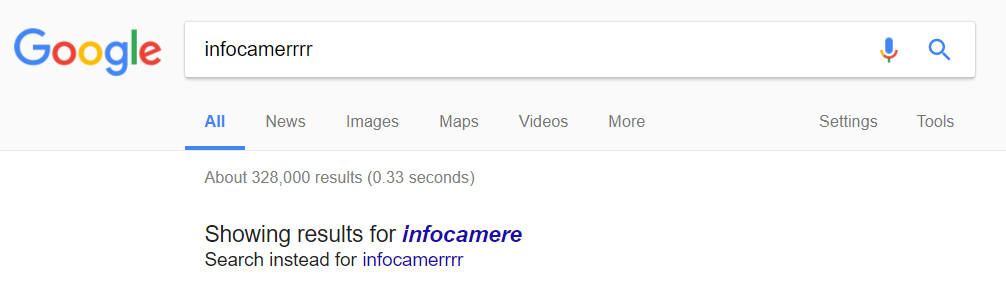
\includegraphics[width=7cm]{did_you_mean}
					\captionof{figure}{Esempio funzionalità "Did you mean...?" in Google}
				\end{center}
			\end{figure}

			\subsubsection{Evidenziamento delle parole ricercate nei risultati}
			Quando vengono ricercati documenti che contengono una quantità significativa di testo, è bene fornire all'utente la possibilità di visualizzare sezioni specifiche di ogni documento, mettendo in risalto le sezioni dei risultati di ricerca contenenti i termini ricercati dagli utenti.
			
			\begin{figure}[htbp]
				\begin{center}
					
\includegraphics[width=7cm]{highlighting}
					\captionof{figure}{Esempio funzionalità di evidenziamento, nei risultati, del termine ricercato}
				\end{center}
			\end{figure}
		
			\subsubsection{Ricerca su file}
			L'utente può trovare, tra i risultati della ricerca che ha effettuato, documenti in vari formati (PDF, doc, ecc...) che contengono le keywords ricercate. Questa funzionalità risulta essere di particolare interesse nell'ambito dei siti informativi Camerali, data la grande mole di dati contenuti in documenti memorizzati in vari formati (prevalentemente PDF).
			
			\begin{figure}[htbp]
				\begin{center}
					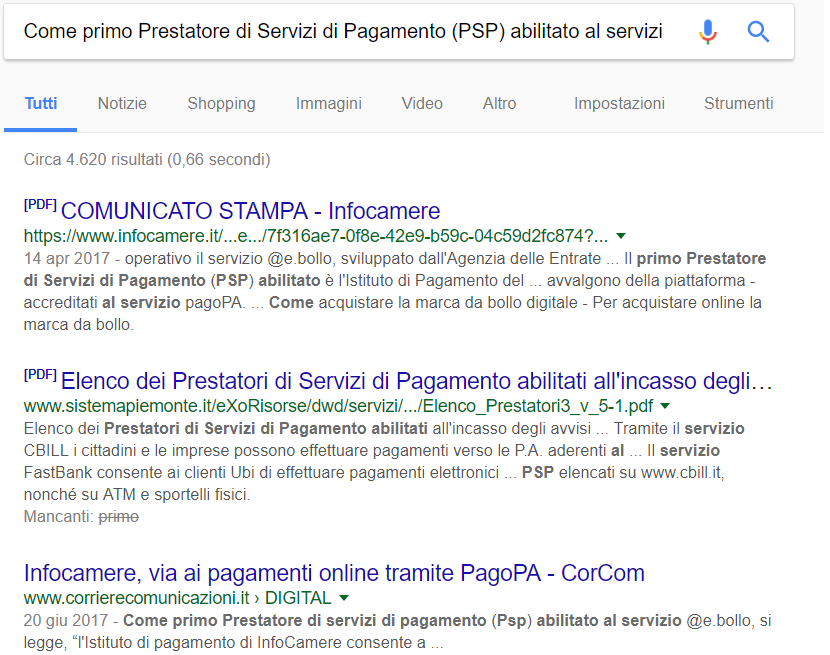
\includegraphics[width=7cm]{ricerca_su_file}
					\captionof{figure}{Esempio funzionalità di ricerca su file offerto da Google}
				\end{center}
			\end{figure}
		
			\subsubsection{Facets}
			Prevalentemente utilizzati nei siti di e-commerce, l'utilizzo di questa funzionalità permette di fornire agli utenti strumenti utili a raffinare le proprie ricerche, ricorrendo a una serie di filtri che consentono di ridurre rapidamente il numero dei risultati di ricerca, selezionando le caratteristiche di interesse di quanto ricercato. In questo modo, l'utente è in grado di costruire il proprio percorso di ricerca, consentendogli di effettuare ricerche più flessibili e che lo aiutino a trovare ciò che sta cercando con poche azioni. \\
			E' di fondamentale importanza che i contenuti siano ben categorizzati, così da permettere all'utente di trovare quanto cercato.
			
			\begin{figure}[htbp]
				\begin{center}
					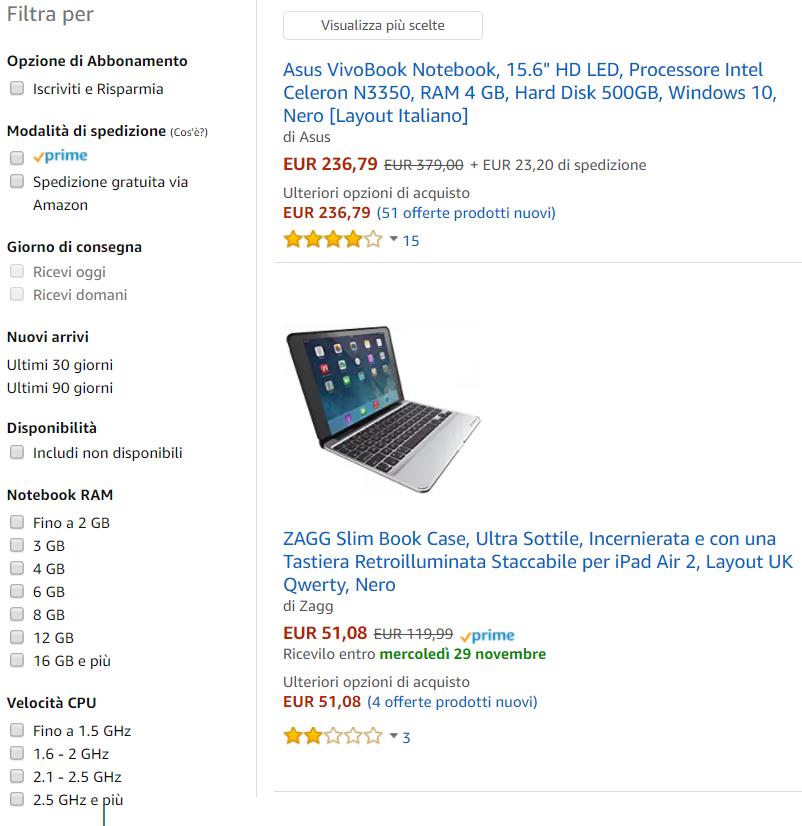
\includegraphics[width=7cm]{facets}
					\captionof{figure}{Esempio funzionalità di filtri multipli (facets) presente su Amazon}
				\end{center}
			\end{figure}
		
			\subsubsection{Importare le funzionalità nei siti informativi Camerali}
			Con l'obiettivo di migliorare la ricerca all'interno dei siti web informativi delle Camere di Commercio, in accordo con il tutor aziendale, abbiamo scelto di concentrare lo studio delle funzionalità offerte dai motori di ricerca oggetto di analisi, principalmente sugli strumenti appena presentati. \\
			Quello a cui vogliamo ambire, è presentato in un prototipo da me creato durante lo stage, contenente alcune delle funzionalità sopra esposti, visibile in \hyperref[img:evoluzioneVR]{Figura 3.9}. \\
			Il prototipo è stato creato con i medesimi dati contenuti nell'attuale sito web informativo della Camera di Commercio di Verona. Il termine ricercato presentato nella figura, è lo stesso della \hyperref[img:conferenze]{ricerca effettuata nell'attuale sito istituzionale camerale di Verona}, ovvero "Conferenze", che non aveva prodotto alcun risultato. Notiamo invece che nel prototipo realizzato, la ricerca del medesimo termine sui medesimi contenuti ha invece prodotto alcuni risultati. Questo è stato possibile migliorando la funzionalità di ricerca, rendendola più flessibile e aumentando la capacità di comprensione del linguaggio naturale.

			\label{img:evoluzioneVR}
			\begin{figure}[htbp]
				\begin{center}
					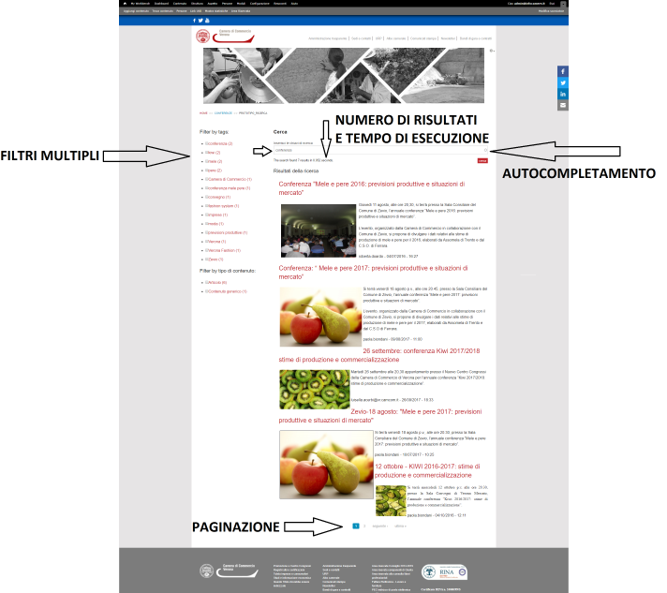
\includegraphics[width=13cm]{vr_futura}
					\captionof{figure}{Possibile evoluzione, mediante aggiunta di funzionalità di ricerca, del sito informativo Camerale di Verona}
				\end{center}
			\end{figure}

	\section{Ricerca nativa Drupal}

		\subsection{Introduzione a Drupal}
		Per arrivare a studiare le funzionalità offerte dai motori di ricerca \gls{Solr} ed \gls{ElasticSearch}, mi sono confrontato con \gls{Drupal}, tecnologia attualmente utilizzata da \nomeAzienda per la creazione dei siti web informativi Camerali. Come viene presentato nella \hyperref[img:cciaa_drupal]{Figura 3.10}, tale tecnologia è l'ambiente con il quale gli utenti comunicano. Le funzionalità di ricerca offerte dai siti creati in \gls{Drupal} possono servirsi di moduli di ricerca internamente presenti all'ambiente, oppure utilizzare connettori in grado di usufruire di motori di ricerca esterni, come possono essere \gls{Solr} ed \gls{ElasticSearch}.
		
		\label{img:cciaa_drupal}
		\begin{figure}[htbp]
			\begin{center}
				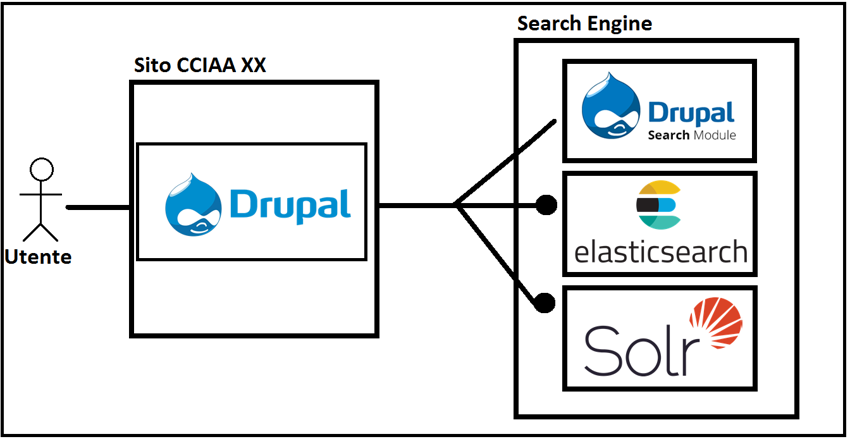
\includegraphics[width=13cm]{cciaa_drupal}
				\captionof{figure}{Utilizzo del motore da parte di un sito Camerale}
			\end{center}
		\end{figure}
	
		Facciamo un passo indietro, e chiediamoci: cos'è Drupal?
		Questa tecnologia è un \gls{CMSg} che permette di creare siti web di vario tipo, rilasciato sotto licenza \gls{open source} e interamente sviluppato in \gls{PHP}, supportando nativamente \gls{MySQL} come base di dati \gls{MySQL}. Inoltre, rappresenta un'applicazione completamente web based, potendo dunque essere utilizzata attraverso un semplice browser. \\		
		L'ambiente \gls{Drupal} mette a disposizione \glspl{Modulo} che consentono di aggiungere funzionalità di ricerca al sito che stiamo realizzando. In particolare, è disponibile una \hyperref[cap:drupalSearch]{ricerca di base e avanzata} e una \hyperref[cap:drupalSearchAPI]{ricerca che sfrutta il modulo Search API offerto da Drupal}, che differiscono tra loro essenzialmente per le funzionalità offerte. Per ognuna di esse, ne ho analizzato le principali caratteristiche, focalizzando l'attenzione sulle funzionalità di possibile interesse per i siti web informativi camerali.
		
			\subsubsection {Scelta della versione Drupal}
			Sono disponibili diverse versioni \gls{Drupal}. Quella utilizzata per tutte le istanze create è la versione 7.56. La scelta deriva dalla volontà di partire da una istanza basilare, contenente solamente i moduli appartenenti al core di questa tecnologia. Esiste inoltre una versione più avanzata, ovvero Drupal 8.x; il motivo per cui la scelta è ricaduta sulla versione 7.x è dato dalla mancanza di moduli aggiornati alla versione 8. Per questo motivo, viene dunque utilizzata una versione più vecchia, della quale sono però presenti un maggior numero di \glspl{Modulo}.
		
		\subsection{Ricerca di base e avanzata}

		\begin{figure}[htbp]
			\begin{center}
				
\includegraphics[width=7cm]{drupal_search_module}
				\captionof{figure}{Ricerca di base e avanzata, offerta dei moduli presenti nel core di Drupal}
			\end{center}
		\end{figure}
	
			\subsubsection{Modalità di operare}
			Per questa tipologia di ricerca, come per tutte quelle che seguono in questo capitolo, ho proceduto innanzitutto alla creazione di una nuova istanza \gls{Drupal}, dedicata alla tipologia di ricerca in esame. Dopo una iniziale configurazione dell'ambiente, ricercando e installando i moduli che mi fornissero le funzionalità di maggior interesse, ho proceduto allo studio delle funzionalità offerte. \\
			Di seguito, riporto le conclusioni emerse dallo studio della ricerca di base e avanzata, resi disponibili dai moduli nativamente contenuti nel core di \gls{Drupal}.

			\subsubsection{Considerazioni sulla ricerca di base e avanzata}
			Una ricerca esaustiva prodotta con questa tecnologia richiede che l'utente conosca esattamente quello che sta ricercando; i contenuti hanno inoltre la necessità di essere fortemente atomizzati e specifici, mediante l'utilizzo di termini significativi, in modo tale da poter essere trovati dall'utente. \\
			Nei siti informativi Camerali, questo limite può essere mitigato ricorrendo all'utilizzo di \gls{Tag}, attraverso la creazione di \glspl{Tassonomia}, in modo da consentire all'utente una navigazione dei contenuti per tag. Così facendo, l'utente dovrà comunque conoscere con esattezza i termini chiave da ricercare e i contenuti dovranno essere etichettati in maniera corretta e specifica per i contenuti. Tutto ciò, porterebbe ad un rapido aumento del numero di tag, rendendo il sistema poco efficiente e fruibile. \\
			Un'ulteriore difficoltà che incontra questo approccio è da ricercarsi nel carico di lavoro che il server sul quale il sito viene ospitato è in grado di gestire. Non essendoci infatti la possibilità di definire engine di ricerca esterni all'ambiente \gls{Drupal}, avendo quindi un database comune, utilizzato anche per effettuare le ricerche, un elevato quantitativo di interrogazioni al database potrebbe causare ritardi significativi o addirittura interruzioni dei servizi offerti dal sito. \\
			Le ricerche di base e avanzata risultano dunque essere primitive, non adatte all'attuale stato di avanzamento tecnologico che si può osservare in vari siti informativi e non adatte a gestire siti di grandi dimensioni, dato lo scarso livello di performance e funzionalità offerte.
		
		\subsection{Ricerca con Search API}
		
			\subsubsection{Modalità di operare}
			Per prima cosa, ho proceduto alla creazione di un'istanza \gls{Drupal} dedicata alla ricerca di con \gls{Search API}.
			Oltre all'installazione di moduli di utilità, non significativi ai fini della ricerca ma che semplificano l'utilizzo dell'intero ambiente di sviluppo, ho installato il modulo \gls{Search API}. \\
			Tale modulo fornisce un \gls{Framework} per creare agevolmente ricerche nell'ambiente \gls{Drupal}, utilizzando qualunque tipologia di motore di ricerca. Prima di arrivare a studiare l'integrazione di questo modulo con i motori \gls{Solr} e \gls{ElasticSearch}, ho sfruttato una ricerca che utilizzasse un \gls{Server} interno all'ambiente \gls{Drupal}, ritrovando ciò nel \gls{Modulo} \gls{Search API Database}.
			Di seguito, riporto le conclusioni emerse dallo studio della ricerca con \gls{Search API} che sfrutta il modulo \gls{Search API Database}.
			
			\subsubsection{Considerazioni sulla ricerca con Search API Database}
			La ricerca \gls{Search API} che utilizza \gls{Search API Database} come \gls{Server} di ricerca, permette di effettuare ricerche in modo molto più flessibile rispetto a quanto offerto dalle ricerche di base e avanzata.
			Questa tecnologia permette un certo grado di complessità nelle stringhe ricercate, offrendo funzionalità molto più adatte alle aspettative degli utenti che navigano il web ai nostri giorni. \\
			\gls{Search API} non supporta tutte le funzionalità offerte dalla ricerca di base e avanzata: in particolare non sono presenti le funzionalità di ricerca che utilizzano clausole condizionali (and, or, not, ...). \\
			Le funzionalità aggiuntive, non presenti nei \glspl{Modulo} contenuti nel core di \gls{Drupal}, consentono però di eseguire ricerche più intelligenti, che aiutano l'utente a trovare contenuti ricercando termini anche non completamente esatti o incompleti. \\
			Le ricerche risultano essere molto più user friendly rispetto a quelle rese disponibili dalla ricerca di base e avanzata, evidenziando un importante passo avanti, date le funzionalità offerte, permettendo agli utenti un margine di flessibilità nei termini ricercati, che non devono dunque conoscere esattamente il termine o il concetto che stanno ricercando. \\
			Il carico di lavoro richiesto dal server sul quale il sito viene ospitato rappresenta un punto critico di questa tecnologia di ricerca: così come per la ricerca di base e avanzata, la ricerca \gls{Search API} che utilizza \gls{Search API Database}, continua a lavorare con un unico database comune, utilizzato anche per effettuare ricerche. Un elevato quantitativo di richieste e l'impossibilità di esternalizzare l'engine di ricerca su macchine che lavorino in modo concorrente potrebbe dunque compromettere i tempi di attesa per ottenere i risultati di ricerca, che diventano critici su siti di grandi dimensioni e con un gran numero di contenuti.

		\subsection{Considerazioni di Drupal nativo}
		la ricerca nativa di \gls{Drupal} permette un gran numero di funzionalità che potrebbero essere di interesse per i siti Camerali. Ulteriori \glspl{Modulo} amplificano inoltre le funzionalità possibilmente utili disponibili mediante l'utilizzo di questa tipologia di ricerca, permettendo funzionalità completamento automatico, paginazione delle ricerche e ordinamento dei risultati di ricerca secondo filtri prestabiliti, "Did you mean...?", evidenziamento dei termini ricercati nei risultati, utilizzo di \glspl{Modulo} per implementare le facets (=filtri multipli), creazione di più \gls{Index} di ricerca e possibilità di effettuare ricerche nei contenuti testuali di alcuni tipi di files (PDF, Word, ecc...). \\
		Questa tecnologia consente dunque di effettuare ricerche con un certo grado di complessità, offrendo funzionalità molto più adatte alle aspettative degli utenti che navigano il web nei nostri giorni. \\
		La ricerca sulle \gls{Stem Words} rappresenta un possibile punto debole di questa tecnologia, non essendo attualmente disponibile un modulo nella versione 7.x per la lingua italiana.\\
		Il carico di lavoro richiesto dal server sul quale il sito viene ospitato rappresenta un punto critico di questa tecnologia. In entrambe le tipologie di ricerca presentate per la ricerca nativa \gls{Drupal}, è presente un unico database comune. Un elevato quantitativo di richieste, unito all'impossibilità di esternalizzare l'engine di ricerca su macchine che lavorino in modo concorrente potrebbe dunque compromettere i tempi di attesa per ottenere i risultati di ricerca, che diventano critici su siti di grandi dimensioni e con un gran numero di contenuti.

	\section{Ricerca con Solr}

		\subsection{Introduzione a Solr}
		
		\begin{figure}[htbp]
			\begin{center}
				
\includegraphics[width=7cm]{logo_solr}
				\captionof{figure}{Motore di ricerca Solr}
			\end{center}
		\end{figure}
	
		\gls{Solr} rappresenta una piattaforma di ricerca \gls{open source}, scritta in \gls{Java}, che viene eseguita come server di ricerca full text indipendente, all'interno di un contenitore \gls{Servlet}. Utilizza \gls{Java Lucene} come libreria per la ricerca e l'indicizzazione full text e mette a disposizione chiamate \gls{REST} come ad esempio, comunicando in vari formati, tra i quali \gls{JSONg} e \gls{XMLg}, rendendo semplice e versatile la comunicazione. \\ Nonostante sia scritto in \gls{Java}, non è necessaria una conoscenza di tale linguaggio per utilizzare questa tecnologia; è inoltre possibile estendere la libreria di ricerca: in questo caso la conoscenza di \gls{Java} risulterebbe, ovviamente, fondamentale. \\
		Questa tecnologia mette a disposizione un gran numero di funzionalità che aiutano l'utilizzatore ad eseguire ricerche semplici e intuitive ma potenti al tempo stesso. E' importante notare che questa tecnologia espone \gls{APIg} che offrono servizi \gls{HTTPg} di tipo \gls{REST}, senza fornire componenti grafici per la ricerca.
		
		\subsection{Principali funzionalità di ricerca}
		
			\subsubsection{Modalità di operare}
			Dopo uno studio iniziale riguardante l'architettura ad alto livello della tecnologia, ho proceduto alla creazione e alla configurazione di una nuova istanza \gls{Solr}; la versione che ho utilizzato è la 5.5.4. Successivamente, ne ho studiato le funzionalità di ricerca più significative offerte dalla tecnologia in esame, prestando attenzione alla sua integrazione con l'ambiente \gls{Drupal}.
			
			\subsubsection{Architettura ad alto livello}
			Per lo studio dell'architettura ad alto livello di questa tecnologia, mi sono servito di letteratura e materiale trovato in rete. Con le fonti trovate, ho individuato le seguenti componenti che vanno a comporre l'architettura di massima di \gls{Solr}, presentate di seguito.
			
			\begin{itemize}
				\label{solr:request_handler}
				\item {\textbf{Request Handler:} Le richieste che arrivano al sistema \gls{Solr} vengono processate da questa componente e possono essere di interrogazione o di aggiornamento dell'\gls{Index}; }
				
				\item{\textbf{Search Components:} Rappresenta l'insieme delle funzionalità di ricerca (faceting, highlighting, more like this, ecc...) offerte da Apache Solr. Le singole componenti di ricerca (search component) si registrano come gestori di ricerca (search handlers). E' inoltre possibile registrare più componenti in un singolo search handler;}
				
				\label{solr:query_parser}
				\item{\textbf{Query Parser:} Il \gls{Parser} di Apache Solr analizza le query passate a \gls{Solr}, verificandone la correttezza sintattica. Successivamente, traduce le interrogazioni in un formato comprensibile a \gls{Java Lucene};}
				
				\item{\textbf{Response Writer:} Componente che si occupa della generazione dell'output a seguito delle interrogazioni eseguite. Vengono supportati vari formati, tra cui \gls{XMLg}, \gls{JSONg}, ecc...;}
				
				\label{solr:analyzer_tokenizer}
				\item{\textbf{Analyzer/tokenizer:} Apache Solr analizza il contenuto e lo divide in \glspl{Token} che verranno successivamente inviati a \gls{Java Lucene}. Un Analyzer esamina il testo dei campi del contenuto e genera un flusso di token. Successivamente, questo flusso di token viene suddiviso in singoli token da un \gls{Tokenizer};}
				
				\item{\textbf{Update Request Processor:} Ogni richiesta di aggiornamento inviata ad Apache Solr passa attraverso una serie di processi, responsabili delle modifiche (eliminazioni, aggiunte di campi, ecc...), che insieme vengono definiti update request processor.}
				
			\end{itemize}
			
			\begin{figure}[p]
				\makebox[\linewidth]{
					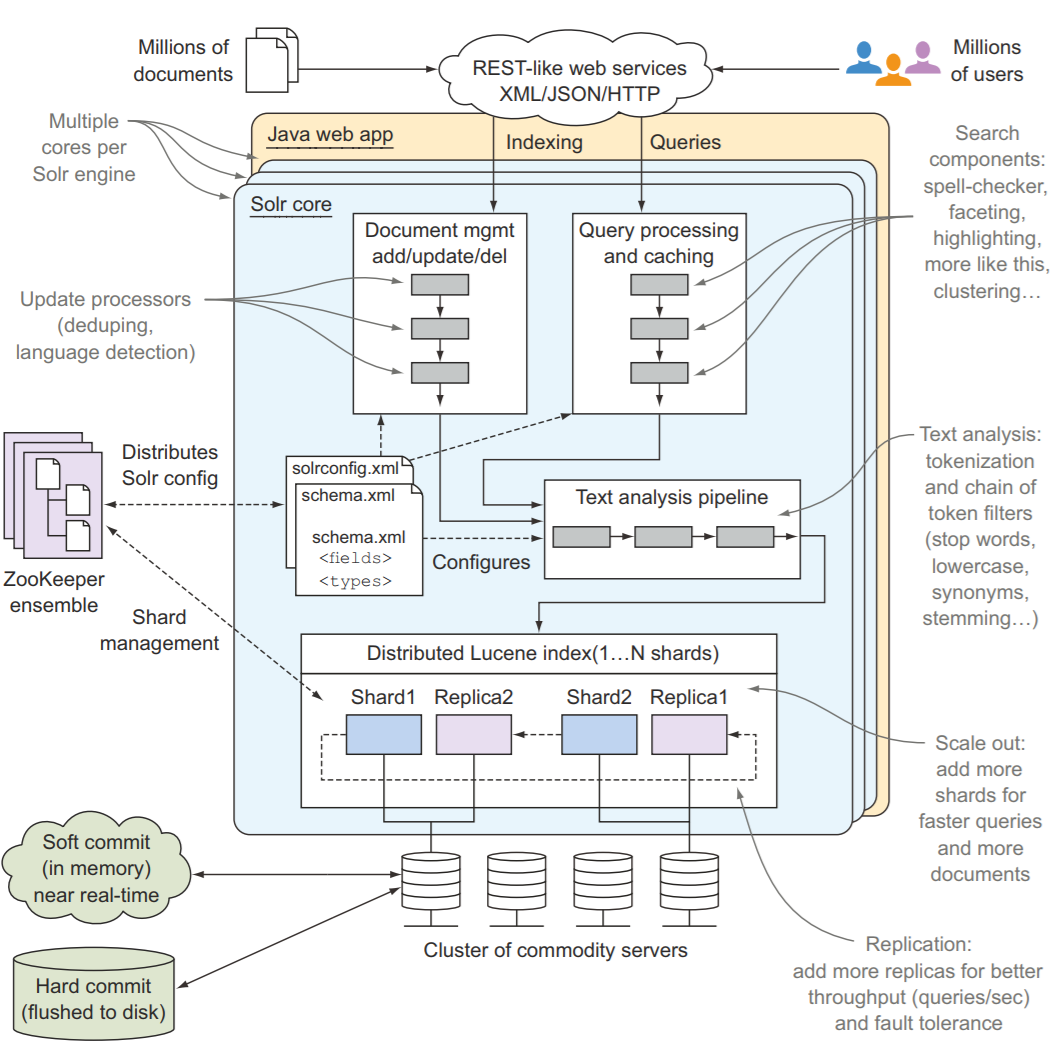
\includegraphics[width=1.3\linewidth]{solr_architettura}
				}
				\caption{Diagramma delle componenti principali di Solr}
			\end{figure}
			
			\subsubsection{Considerazioni sulla ricerca Solr}
			Per ogni tipologia di funzionalità di interesse per i siti informativi Camerali, ho proceduto alla configurazione delle componenti in modo tale da creare esempi funzionanti che supportassero la funzionalità in esame. In particolare, ho potuto constatare che tutte le funzionalità di possibile interesse per \nomeAzienda, presentate in \hyperref[sub:possibile_evoluzione]{3.3.2}, vengono offerte e supportate da \gls{Solr}. \\
			Lo step successivo, consisteva nel verificare se tali funzionalità continuavano ad essere supportate integrando questo motore di ricerca con l'ambiente \gls{Drupal}, in quanto quest'ultimo avrebbe potuto agire da collo di bottiglia.

		\subsection{Integrazione con Drupal}
		Le versioni di \gls{Drupal} (7.56) e di \gls{Solr} (5.5.4) utilizzate permettono l'integrazione di queste due tecnologie in due differenti modalità, presentate di seguito.
		
			\subsubsection{Apache Solr}
			Apache Solr permette di integrare il motore di ricerca \gls{Solr} con l'ambiente \gls{Drupal} mediante utilizzo di un apposito \gls{Modulo}, denominato "Apache Solr". Questo modulo mette in comunicazione il modulo di ricerca "Search" offerto dal core di \gls{Drupal} con il motore di ricerca. \\
			Dopo aver creato e configurato un'apposita istanza \gls{Drupal} che utilizzasse il suddetto modulo, ho potuto constatare che, pur utilizzando un potente motore di ricerca, non vengono supportate alcune delle funzionalità di possibile interesse per i siti Camerali, data l'assenza di \glspl{Modulo} necessari all'integrazione della ricerca di base e avanzata con \gls{Solr}. In particolare, un'istanza \gls{Drupal} che utilizzi il modulo "Apache Solr" non permette l'utilizzo dei filtri multipli nè la creazione di più indici, utili per gestire tipologie di ricerca che differiscano per tipo di documento/entità ricercata, all'interno di un sito.
			
			\subsubsection{Search API Solr}
			Search API Solr permette di integrare il motore di ricerca \gls{Solr} con l'ambiente \gls{Drupal} utilizzando il modulo "Search API Solr", che funge da connettore tra le due tecnologie, mettendo in comunicazione il modulo di ricerca \gls{Search API} con il motore di ricerca. \\
			Dopo aver creato e configurato un'apposita istanza \gls{Drupal} che utilizzasse il suddetto modulo, ho avuto modo di vedere che tutte le funzionalità di possibile interesse per i siti Camerali vengono ben supportate da questa tipologia di integrazione, risultando essere lo strumento di maggior interesse tra tutti quelli presentati fino ad ora.
	
	\section{Ricerca con ElasticSearch}
	
		\subsection{Introduzione a ElasticSearch}
		Qui verrà introdotto ElasticSearch, spiegando cos'è e come funziona.
		%Ranking

		\subsection{Principali funzionalità di ricerca}
		Qui verranno presentate le principali funzionalità di ricerca offerte dal motore di ricerca ElasticSearch, di possibile interesse per i siti camerali.
		
		\subsection{Integrazione con Drupal}
		Qui verranno discusse le funzionalità di ricerca derivanti dall'integrazione tra ElasticSearch e Drupal.
		%Accenno alla versione Drupal8?
		
			\subsubsection{Search API ElasticSearch}
			Qui verranno discusse le funzionalità di ricerca derivanti dall'integrazione tra ElasticSearch e Drupal mediante il modulo Search API ElasticSearch.
			
	\section{Considerazioni finali sui motori di ricerca esaminati}
	Questa sezione conterrà un confronto tra le principali funzionalità, possibilmente di interesse per l'azienda, offerte dalle tecnologie esaminate e quale di queste potrebbe essere la più adatta ai siti camerali.